\section{Experimentación}
A continuaci\'on analizaremos los distintos aspectos de la resoluci\'on implementada para la segmentaci\'on. Debido a las características del problema, la discusi\'on se centrar\'a en dos ejes principales: como esta es una implementaci\'on particular debemos considerar su eficiencia y las propiedades que posee midiendo las métricas correspondientes. Por otro lado, como se present\'o en la introducci\'on, este problema carece de una respuesta objetiva y absoluta, por lo tanto se buscar\'a dar cierto parámetro del objetivo buscado y responder si el algoritmo lo satisface. \\
\indent Específicamente los experimentos realizados consisten en comparar el efecto que tienen las distintas estructuras planteadas en la secci\'on de desarrollo y justificar la complejidad temporal propuesta. Luego analizaremos si la funci\'on de \textit{threshold} planteada en \cite{Felzenszwalb2004} cumple la propiedad propuesta. Hechas estas consideraciones buscaremos dar una respuesta a cu\'al es la calidad de la segmentaci\'on utilizando un \textit{dataset} con su correspondiente \textit{groundtruth}. Por último veremos c\'omo se comporta el algoritmo frente a distintas posibles aplicaciones y se intentara determinar si es apto para alguna de ellas.      

\subsection{Comparaci\'on de las estructuras}
Como se explic\'o en la secci\'on de implementaci\'on, para realizar ciertas operaciones en el algoritmo\ref{segmentation}, es necesario utilizar un tipo abstracto de datos \textit{Disjoint Set}. Se mostr\'o que este pod\'ia ser implementado de al menos tres formas distintas y se justificaron las complejidades. Ahora vamos a evaluar cuál es el rendimiento del algoritmo utilizando las distintas estructuras posibles.\\
\indent Para este experimento se tom\'o una imagen original de dimensiones de $1240\times 960$ píxeles a la cual se la redimension\'o a distintos tama\~nos. Luego se ejecut\'o el algoritmo para cada imagen y se midi\'o el tiempo en realizar únicamente la segmentaci\'on, ya que se consider\'o que la lectura de la imagen y la generaci\'on de las aristas era constante para las tres versiones. Además para este experimento se considera que tanto el contenido de la imagen original como el valor de $k$ es irrelevante al tiempo que toma la ejecuci\'on.\\
\indent Basado en lo discutido sobre el an\'alisis te\'orico del costo, se esper\'o que la estructura que tarde m\'as tiempo sea el arreglo de representantes, seguido del arbol de representantes y luego la versi\'on con \textit{path relinking}. Esto se justifica en el hecho de que los \textit{unite} del arreglo tardan estrictamente $n$ pasos, mientras que en este contexto para los arboles de representantes esta operaci\'on se realiza en tiempo constante. Además el uso de \textit{path relinking} tiene un costo te\'orico menor al de las otras dos opciones, por lo tanto explicar\'ia que sea la versi\'on optima respecto al resto.
\vspace{-3mm}
\begin{figure}[H]
\begin{center}
	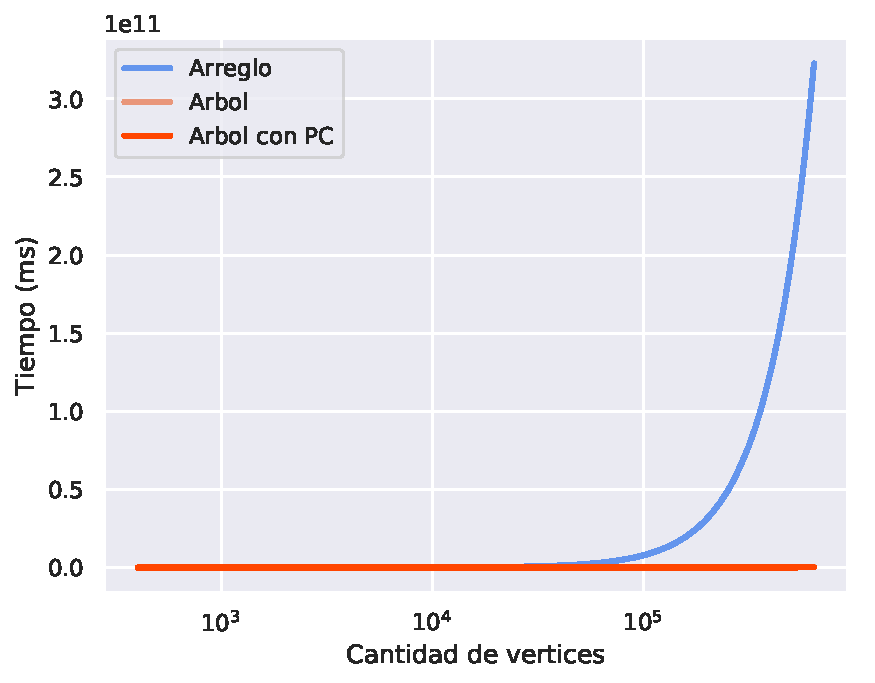
\includegraphics[scale=0.5]{plots/compEstr.pdf}
	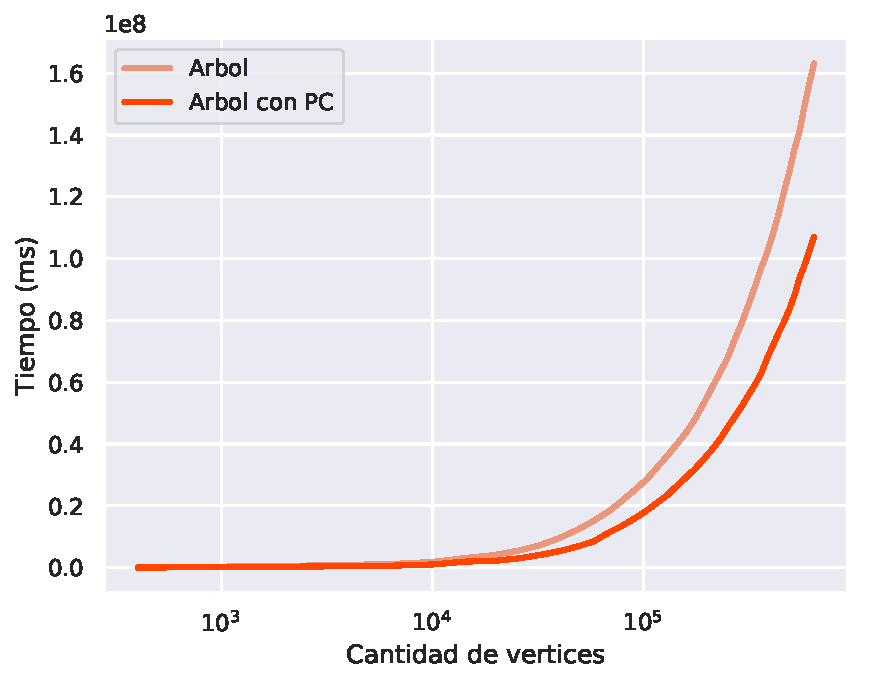
\includegraphics[scale=0.5]{plots/comp_arbs.pdf}
	\caption{Comparaci\'on de tiempos para las distintas estructuras. La cantidad de vértices es de $(20p)^2$ con $p\in[1,40]$ y $k=1000$.}
	\label{comp_estr}
\end{center}
\end{figure}
\vspace{-7mm}

\indent Efectivamente se cumpli\'o experimentalmente lo que se esperaba en base al costo te\'orico. Podemos ver como el ritmo de crecimiento que conlleva utilizar el arreglo de representantes supera vastamente al de los árboles, debido a esto es necesario visualizar por separado el rendimiento de las estructuras de árboles. En el segundo gr\'afico se ve como para instancias de tama\~no mayor sí aparenta haber una notable diferencia entre las opciones, sin embargo no parecer\'ia que utilizar árbol de representaci\'on tenga un ritmo de crecimiento muy distinto a la versi\'on con \textit{path relinking}, sino más bien que hay una diferencia en la constante de multiplicaci\'on. Un experimento posible que no se realiz\'o es comprobar si en la práctica y para esta aplicaci\'on usar un árbol de representantes implica un costo lineal del algoritmo. Esto último no se comprob\'o ya que, aunque llegue a ser cierto, sigue siendo conveniente utilizar \textit{path relinking}.

\subsubsection{An\'alisis temporal del algoritmo}
Habiendo hecho la comparaci\'on en el experimento anterior y habiendo decidido que utilizar \textit{path relinking} era ventajoso, se propuso medir el tiempo de la totalidad del procedimiento esta vez teniendo en cuenta el costo de conseguir el grafo a partir de la imagen. Esto resulta de interés ya que al fin y al cabo el procedimiento en su totalidad es lo que verdaderamente se quiere saber si es eficiente o no. Para esto se tomó el mismo conjunto de im\'agenes propuesto para el experimento anterior y el mismo valor de $k$. El objetivo es mostrar empíricamente que el costo total de todo el algoritmo es de $\mathcal{O}(n)$. \\
\indent Con fines de justificar esta afirmaci\'on se utiliz\'o la teor\'ia de \textit{cuadrados m\'inimos lineales}:\\
\indent Poseemos una muestra de valores de tiempo en funci\'on del tama\~no de entrada $(n_1, t_1) \dots (n_k, t_k)$ y queremos aproximarlos con una funci\'on $f \in F$ familia de funciones, de forma que $f$ minimice la expresión: 
\[
	\sum_{i=1}^k(f(n_i)-t_i)^2
\]
Esta teor\'ia nos es útil pues podemos tomar la familia de funciones $F: \ an+b$. Luego la teor\'ia nos asegura que siempre podemos determinar los coeficientes $a$ y $b$ que minimizan la expresi\'on. Esto nos es ventajoso pues de esta forma encontramos una funci\'on que pertenece al supuesto orden del peor caso de nuestro algoritmo y que además minimiza el criterio de cuadrados m\'inimos.  
Luego de haber conseguido estos coeficientes (y por lo tanto la funci\'on) podemos utilizar la \textit{fórmula de Pearson} sobre las muestras $(n_1, t_1) \dots (n_k, t_k)$ y $(n_1, f(t_1)) \dots (n_k, f(t_k))$ y as\'i obtener una m\'etrica sobre el grado de correlaci\'on entre los datos y la funci\'on. 
\begin{figure}[H]
	\begin{center}
		\subfigure[Comparaci\'on de tiempo de ejecuci\'on y costo te\'orico]{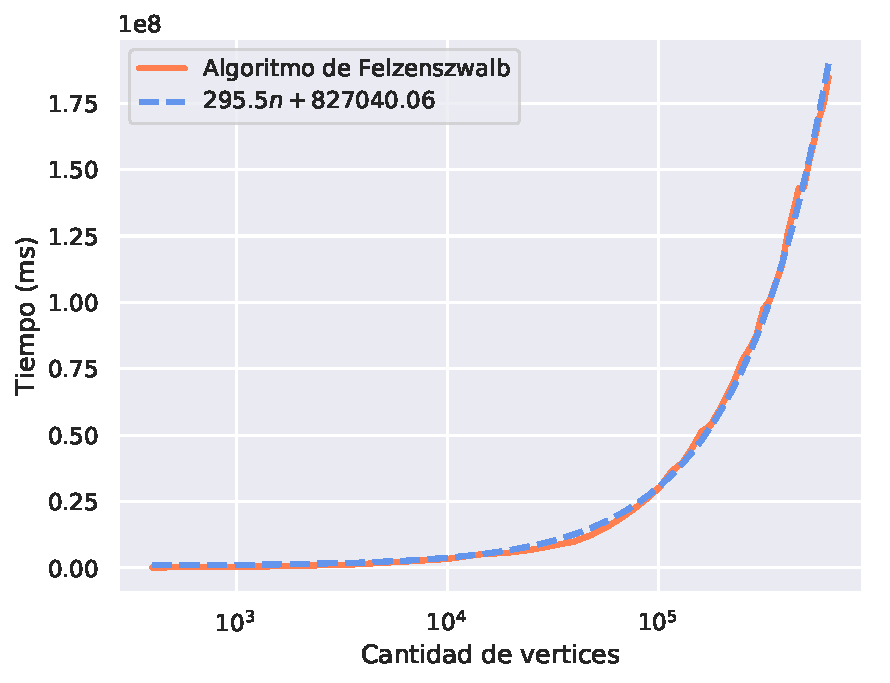
\includegraphics[scale=0.5]{plots/tiempo_Felzen.pdf}}
		\subfigure[Correlaci\'on entre el algoritmo y el costo te\'orico]{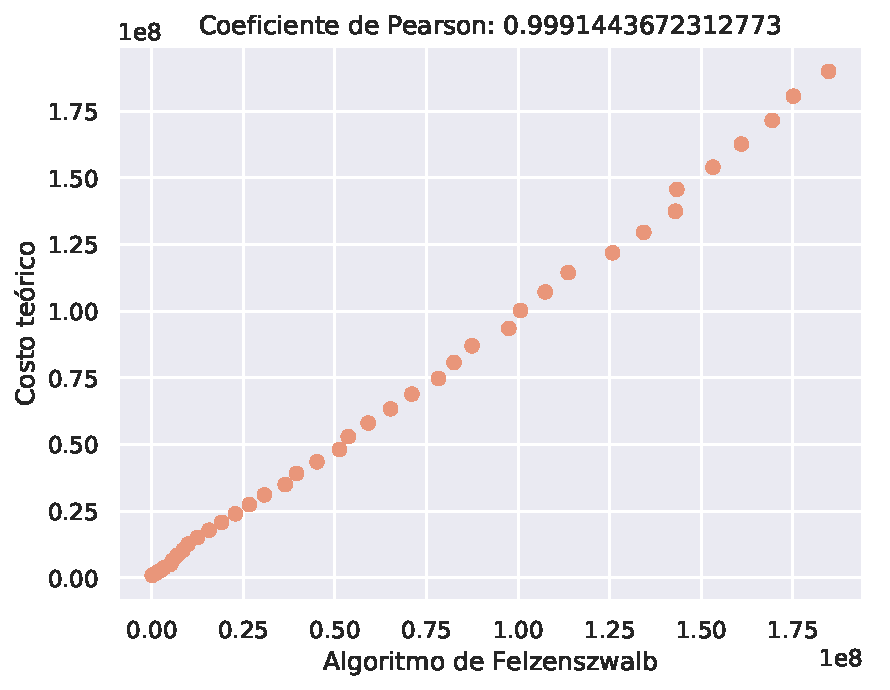
\includegraphics[scale=0.5]{plots/Felzen_corr.pdf}}
		\label{costo_teo}
	\end{center}
	\caption{}
\end{figure}
\vspace{-7mm} 

\indent Como era esperado los datos obtenidos soportan la complejidad te\'orica propuesta, dejando en claro que el algoritmo implementado es eficiente para el problema a resolver. 


\subsection{Influencia de $k$ sobre la granularidad del resultado}
En el trabajo \cite{Felzenszwalb2004} se toma la funci\'on de \textit{threshold} $\tau(C)=\frac{k}{\#C}$ con $k$ un hiperparámetro. Intuitivamente podemos ver que un $k$ menor da lugar a componentes más chicas y análogamente un $k$ mayor tiende a unir componentes, ya que afecta directamente sobre el predicado que da evidencia si hay un l\'imite entre componentes. El objetivo del siguiente experimento es buscar una correlaci\'on empirica entre esta noci\'on y las segmentaciones resultantes. \\
Para poder dar una afirmaci\'on estadisticamente robusta se utiliz\'o el \textit{Berkeley Segmentation Dataset} (BSDS) \cite{BSDS} que consiste en 300 im\'agenes variadas. Luego se comput\'o la segmentaci\'on para cada valor de $k$ y para cada imagen, midiendos\'e la cantidad de componentes distintas. 

\begin{figure}[H]
	\begin{center}
	\subfigure[Imagen de ejemplo perteneciente al BSDS]{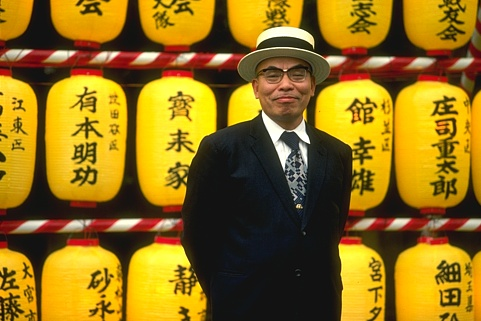
\includegraphics[scale=0.35]{segmentaciones/sr.jpg}}
	\hspace{5mm}
	\subfigure[Cantidad de componentes para distintos $k$]{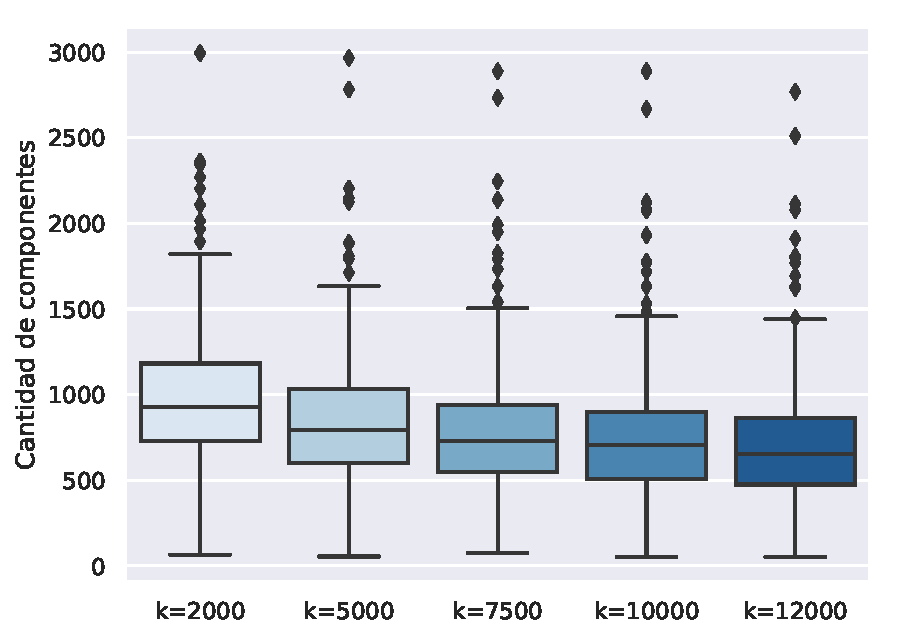
\includegraphics[scale=0.5]{plots/boxplot_k.pdf}}
	\caption{}
	\end{center}
	\label{comp_k}
\end{figure}
\vspace{-7mm} 

\indent Como podemos observar en la figura 4 \textit{(b)}, a medida que se aumenta el $k$ la media de componentes disminuye. Además las relaciones de los cuartiles no son afectadas, lo que lleva a pensar que para todas las imagenes la influencia del valor de $k$ afecta de manera similar.

\begin{figure}[H]
	\begin{center}
	\subfigure[$k=2000$]{
\includegraphics[scale=0.35]{segmentaciones/sr-2000.jpg}}
	\hspace{1mm}
	\subfigure[$k=5000$]{
\includegraphics[scale=0.35]{segmentaciones/sr-5000.jpg}}
	\hspace{1mm}
	\subfigure[$k=7500$]{
\includegraphics[scale=0.35]{segmentaciones/sr-7500.jpg}}
	\hspace{1mm}
	\subfigure[$k=10000$]{
\includegraphics[scale=0.35]{segmentaciones/sr-10000.jpg}}
	\hspace{1mm}
	\subfigure[$k=12000$]{
\includegraphics[scale=0.35]{segmentaciones/sr-12000.jpg}}
	\caption{}
	\end{center}
	\label{costo_teo}
\end{figure}
\vspace{-7mm} 

\indent En la foto usada de ejemplo podemos ver efectivamente el efecto de incrementar al hiperparámetro. En un principio los rasgos faciales son m\'as faciles de distinguir y los kanjis en las linternas no fueron todav\'ia considerados como el interior del objeto. Al mismo tiempo se ve mucha variabilidad en zonas que se esperar\'ian uniformes como el saco. A medida que se incrementa el valor vemos como se alisan ciertas secciones, ganando mayor definici\'on y separaci\'on pero algunos detalles como los ideogramas se pierden. Ya para los últimos casos los contornos generales quedan mayormente separados con muy pocos detalles peque\~nos distinguibles. Notar que estas últimas generalizaciones a componentes m\'as grandes puede traer uniones no deseadas, como es el caso del cuello de la camisa en este ejemplo: para $k=5000$ hay una distinci\'on con la lampara que interseca con la camisa, pero para todos los valores de $k$ siguientes estas dos regiones se unen.\\
\indent Este experimento confirma la intuici\'on original sobre los efectos del hiperparámetro $k$ y se tendrán en cuenta para la experimentaci\'on siguiente.


\subsection{Calidad de la segmentaci\'on}
Si bien el objetivo de resolver el problema es dar una segmentaci\'on que refleje los objetos de interés en una imagen, como ya se mencion\'o, esto es completamente subjetivo. Principalmente hay dos partes fundamentales a esta subjetividad, una siendo que es lo que se quiere estudiar de un conjunto de imágenes (cual es el objeto de interés) y la otra respecta al observador de la imagen segmentada (quien aprueba el resultado). Aunque este sea el caso no quita que sea de interés poder dar una respuesta a la pregunta de cu\'an buena es una segmentaci\'on. \\
\indent Con este objetivo se consider\'o utilizar un \textit{data set} que posea la \textit{ground truth} de las segmentaciones: segmentaciones fabricadas por humanos que se consideraran como la respuesta objetivamente correcta al problema. Se utiliz\'o un subconjunto del BSDS presentado en \cite{li2013benchmark} en el cual se propone una construcci\'on del \textit{ground truth} basada en niveles de percepción de la imagen y consideran que su objeto de estudio son las figuras contrastantes con los distintos fondos de la imagen original. A grandes rasgos consideran que la segmentaci\'on debe ser gruesa y bien definida. \\
\indent A partir de este \textit{data set} se implement\'o una comparaci\'on entre las imágenes \textit{ground truth} y la segmentaci\'on obtenida. La m\'etrica considerada fue el $F_2$ score:
\[
	F_2 = (1+2^2)\frac{\text{Precision}\times{Recall}}{2^2\times \text{Precision}+\text{Recall}}
\]
\indent En este contexto \textit{Precision} significa saber de todos los píxeles que la segmentaci\'on clasifico en la misma componente, cuantos verdaderamente lo estaban. \textit{Recall} representa cuántas asociaciones correctas se hicieron. Por el problema a resolver y las consideraciones hechas en \cite{Felzenszwalb2004} se consider\'o darle mayor importancia al valor de \textit{Recall} para reforzar el peso de los \textit{falsos negativos}: poner un l\'imite entre dos componentes cuando no lo hay. Con esto se justifica usar $\beta =2$ para el $F_{\beta}$ score.\\
\indent Para cada píxel $P_i$ se consider\'o su \textit{k-ring} de píxeles $P_j$, comparando para cada par si pertenecían o no a la misma componente en la segmentaci\'on obtenida y en la \textit{ground truth}. Con esto se obtienen los valores de \textit{true positives, false positives, true negatives} y \textit{false negatives}. En la experimentaci\'on se consider\'o el \textit{5-ring}, con la justificaci\'on que este radio proporcionar\'ia suficiente informaci\'on local (contexto del píxel $i$). \\
\indent Como las componentes que se generan son de gran tama\~no, hacer el procedimiento para todo pixel desbalancear\'ia la cantidad de \textit{true positives}. Esto se debe a que se tendr\'ian en cuenta grandes porciones lisas de la imagen y estas no proporcionan gran informaci\'on sobre los puntos de interés (los l\'imites). Por lo tanto se tuvo en cuenta \'unicamente los píxeles ``borde'' de la segmentaci\'on obtenida. Esto mide mejor lo propuesto ya que si un píxel es de ``borde'' en la imagen obtenida pero no lo es en la \textit{ground truth} aumentarán los \textit{false positives} que es justamente lo que se considera importante de captar.

\begin{figure}[H]
	\begin{center}
	\subfigure[$F_2$ scores para el data set]{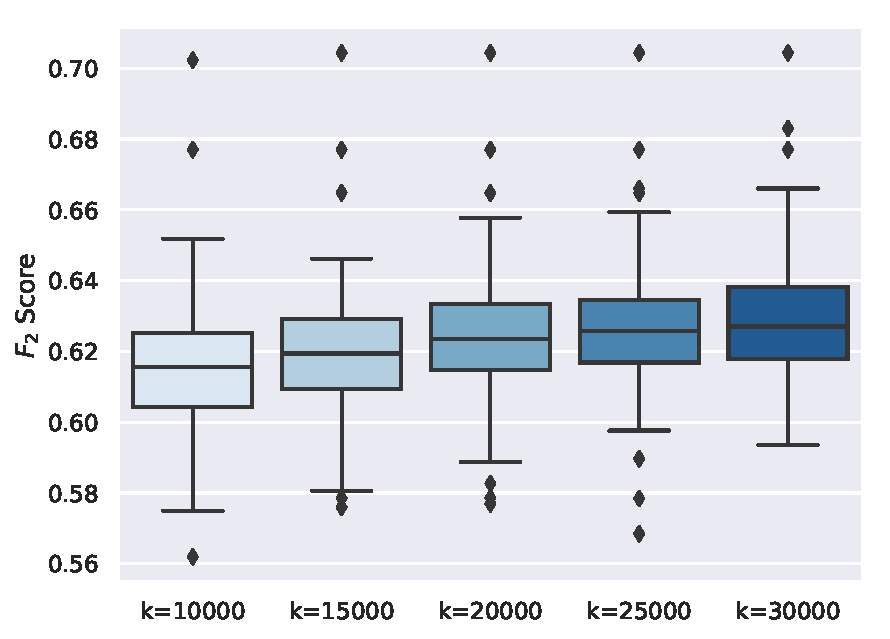
\includegraphics[scale=0.5]{plots/fScores_k.pdf}}
	\hspace{3mm}
	\subfigure[Desviaci\'on estandar de la m\'etrica]{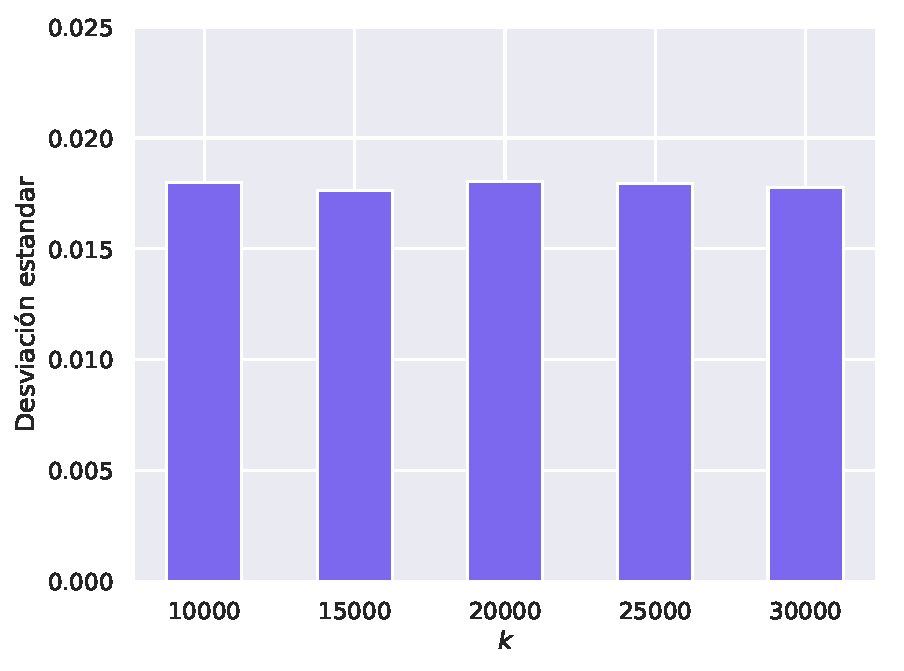
\includegraphics[scale=0.5]{plots/std_k.pdf}}
	\caption{}
	\end{center}
	\label{Fscores}
\end{figure}
\vspace{-7mm} 

\indent En primer lugar se observa que si bien hay una mejora en la calidad de segmentaci\'on a medida que se toma un $k$ mayor, este incremento es relativamente peque\~no ya que las medias de $k=10000$ y $k=30000$ difieren en no m\'as de $0.04$. A su vez, la variabilidad que presenta el data set es muy peque\~na, como se puede observar en el gr\'afico de barras. Intuitivamente esto sugiere que la segmentaci\'on funciona con la misma calidad sin importar la imagen sobre la que se utilize.\\
\indent Se puede observar que para todos los valores de $k$ utilizados hay un \textit{outlier} con un valor de aproximadamente $0.7$, se comprob\'o que este siempre se corresponde a la misma imagen que se expone a continuaci\'on:
\begin{figure}[H]
	\begin{center}
	\subfigure[Imagen original]{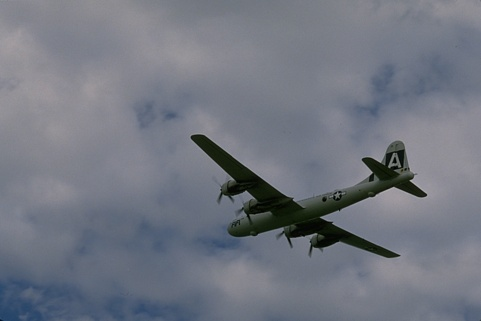
\includegraphics[height=120pt, width=140pt]{segmentaciones/3096.jpg}}
	\hspace{3mm}
	\subfigure[Ground truth]{
\includegraphics[height=120pt, width=140pt]{segmentaciones/3096.png}}
	\hspace{3mm}
	\subfigure[Segmentaci\'on ($k=30000$)]{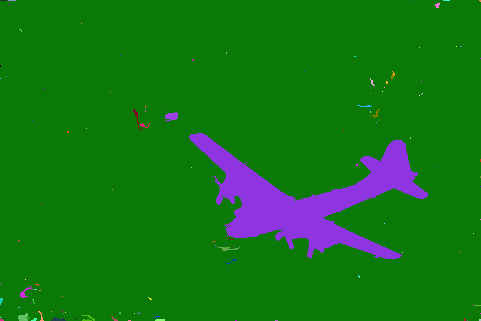
\includegraphics[height=120pt, width=140pt]{segmentaciones/3096_seg.jpg}}
	\caption{}
	\end{center}
	\label{Fscores}
\end{figure}
\vspace{-7mm} 
No es sorprendente que una imagen de esta índole, cuyos contornos son fáciles de distinguir y con iluminaci\'on uniforme, sea la que produzca un mejor resultado. De todas formas el algoritmo sigue siendo susceptible a ciertos patrones como el cambio entre cielo y nubes, que le agregan ruido indeseado. Queda como trabajo futuro analizar si con esta implementaci\'on es posible modificar la funci\'on $\tau$ para evitar este comportamiento. Notar que si no se tomase como restricci\'on considerar \'unicamente los píxeles ``borde'' im\'agenes como esta tendr\'ian valores de \textit{Precision}$\approx 1$ debido a la gran componente del fondo. \\
\indent A su vez podemos observar la imagen que para la mayor\'ia de los valores de $k$ obtuvo el peor valor de $F_2$
\begin{figure}[H]
	\begin{center}
	\subfigure[Imagen original]{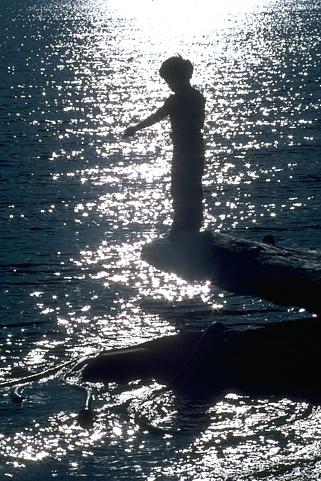
\includegraphics[height=120pt, width=140pt]{segmentaciones/26031.jpg}}
	\hspace{3mm}
	\subfigure[Ground truth]{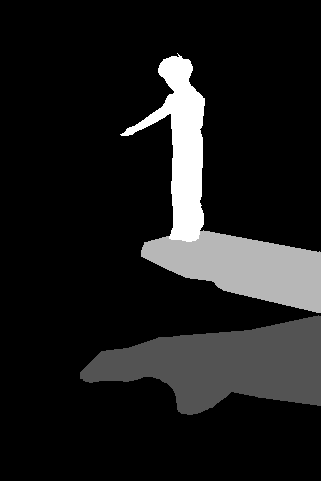
\includegraphics[height=120pt, width=140pt]{segmentaciones/26031.png}}
	\hspace{3mm}
	\subfigure[Segmentaci\'on ($k=30000$)]{
\includegraphics[height=120pt, width=140pt]{segmentaciones/26031_seg.jpg}}
	\caption{}
	\end{center}
	\label{Fscores}
\end{figure}
\vspace{-7mm} 

\indent Esta presenta muchos problemas para nuestro algoritmo por la alta variabilidad de colores que genera la luz. Es argumentable que el objeto de interés de esta imagen es el sujeto erguido, y en segundo plano las rocas y el agua. El algoritmo junt\'o al sujeto y las rocas mientras que el agua la separo basado en la iluminaci\'on que esta recible. Se podr\'ia decir que para este tipo de fotos la segmentaci\'on no es la esperada.
 

\subsection{Distintas aplicaciones y an\'alisis cualitativo}
Si bien el algoritmo es correcto respecto a su especificaci\'on y cumple las propiedades propuestas, el objetivo de la segmentaci\'on es poder diferenciar un objeto de estudio para un conjunto de im\'agenes que cumplen alguna particularidad. A continuaci\'on se tuvieron en cuenta distintos problemas que se pueden resolver utilizando segmentacion de im\'agenes y se evalu\'o si el algoritmo implementado pudiese ser de utilidad para estos casos.

\subsubsection{Reconocimiento de transeúntes}
Una de las nuevas tecnolog\'ias en desarrollo es la de autmóviles autónomos. Uno de los desaf\'ios que presenta es el reconocimiento de sujetos en la calle, a fin de evitar accidentes. En parte este problema se podr\'ia resolver utilizando una segmentaci\'on en tiempo real, junto con un clasificador del objeto segmentado. \\
Tomando im\'agenes de la \textit{Penn-Fudan Database for Pedestrian Detection and Segmentation} \footnote{\url{https://www.cis.upenn.edu/~jshi/ped_html/#pub1}} podemos evaluar el comportamiento del algoritmo sobre instancias reales.
\begin{figure}[H]
	\begin{center}
	\subfigure[]{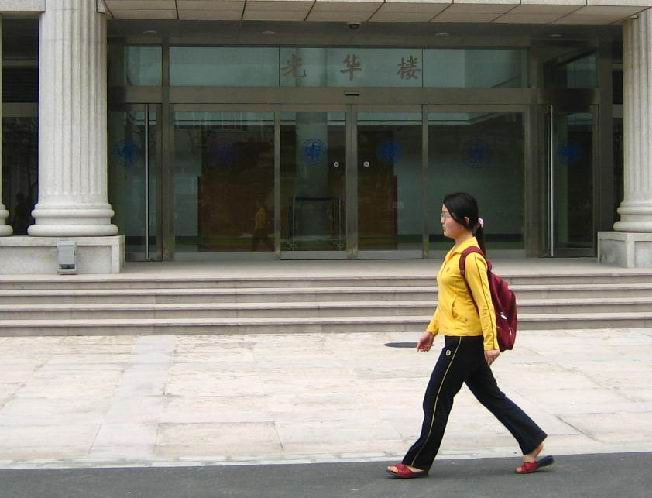
\includegraphics[height=110pt, width=110pt]{segmentaciones/call1.jpg}}
	\subfigure[$k=12000$]{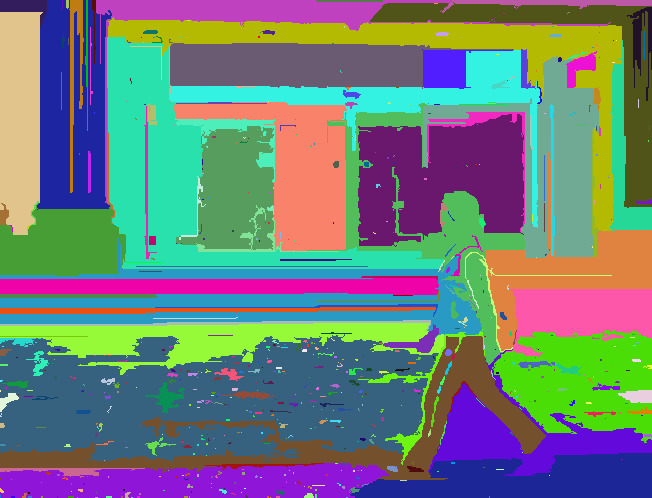
\includegraphics[height=110pt, width=110pt]{segmentaciones/call1_seg.jpg}}
	\hspace{3mm}
	\subfigure[]{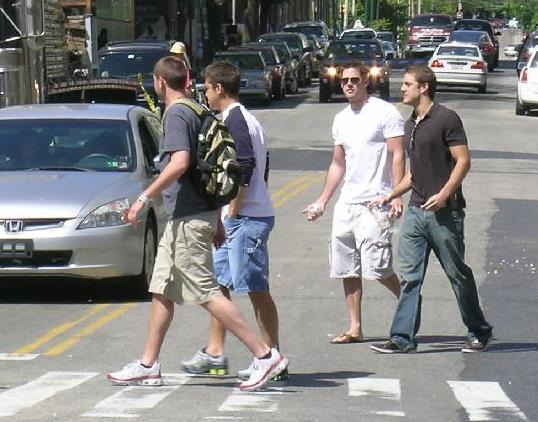
\includegraphics[height=110pt, width=110pt]{segmentaciones/call2.jpg}}
	\subfigure[$k=12000$]{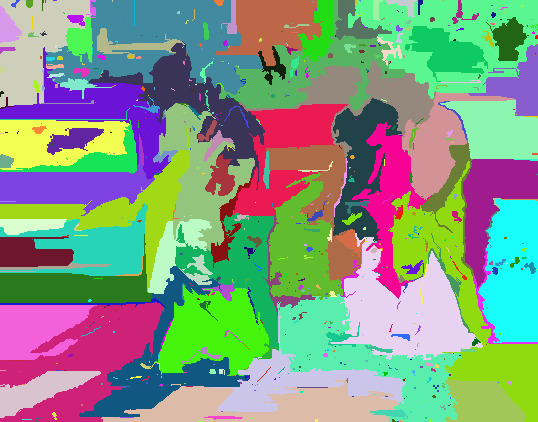
\includegraphics[height=110pt, width=110pt]{segmentaciones/call2_seg.jpg}}
	\caption{}
	\end{center}
	\label{Rec_tran}
\end{figure}
\vspace{-7mm}

\indent Evidentemente el comportamiento no es el requerido, mucha informaci\'on de los fondos afecta negativamente sobre el objeto de estudio y no es distinguible fácilmente. Se podr\'ia considerar tomar un valor de $k$ mayor, pero esto tampoco funcionar\'ia ya que en la subfigura \textit{(b)} ya hay componentes que son la junta de dos partes distintas, como es el caso de la mochila y las escaleras del fondo. Mismo en la subfigura \textit{(d)} la mayor parte de las cosas es irreconocible en la segmentaci\'on.

\subsubsection{Divisi\'on de rasgos faciales}
En varias aplicaciones puede ser de interés reconocer rasgos faciales de un individuo, como por ejemplo en filtros de im\'agenes hasta reconocimiento de gente desaparecida. Tomando algunas fotos de un \textit{dataset} \footnote{\url{http://pics.psych.stir.ac.uk/2D_face_sets.htm}} podemos analizar el comportamiento de las segmentaciones.
\begin{figure}[H]
	\begin{center}
	\subfigure[]{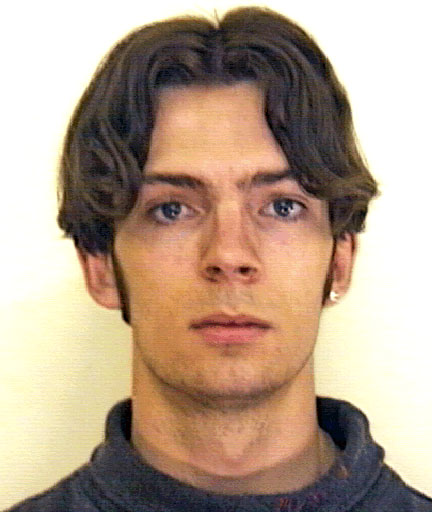
\includegraphics[height=110pt, width=110pt]{segmentaciones/cara1.jpg}}
	\subfigure[$k=10000$]{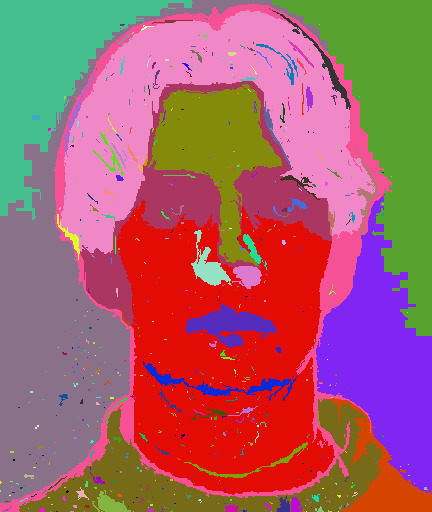
\includegraphics[height=110pt, width=110pt]{segmentaciones/cara1_seg.jpg}}
	\hspace{3mm}
	\subfigure[]{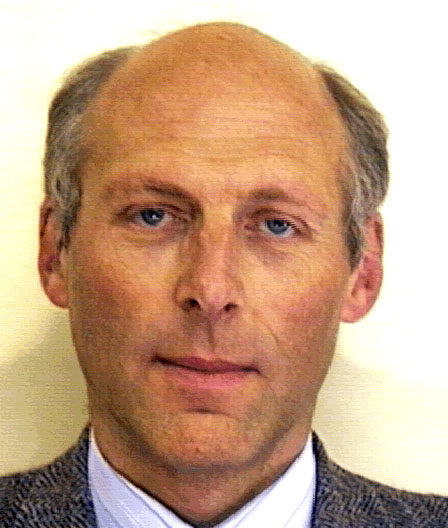
\includegraphics[height=110pt, width=110pt]{segmentaciones/cara2.jpg}}
	\subfigure[$k=10000$]{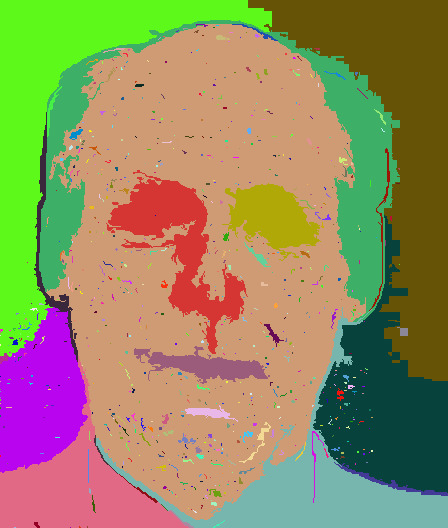
\includegraphics[height=110pt, width=110pt]{segmentaciones/cara2_seg.jpg}}
	\caption{}
	\end{center}
\end{figure}
\vspace{-7mm}

\indent En comparaci\'on' al problema de reconocimiento de transeúntes, el algoritmo parece funcionar mejor para esta tarea. Vemos como ciertos aspectos como el pelo de las personas se encuentra bien delimitado, las bocas se pueden distinguir aunque con algo de ruido y partes como los ojos quedan sumidos en otras componentes. Si bien no parecer\'ia ser aplicable al problema propuesto, el rendimiento parece mejorar para este problema que se podr\'ia decir m\'as simple.  


\subsubsection{Identificaci\'on de núcleos celulares}
Uno de los ambientes en donde m\'as se trabaja con procesamiento de im\'agenes digitales es en el \'area de la medicina.  Reconocimiento de tejidos, tumores y separaci\'on de celulas de im\'agenes microscópicas son algunas de las tareas que se resuelven al d\'ia de hoy, aunque generalmente con un acercamiento desde lo que se conoce como \textit{machine learning}. \\
\indent De un \textit{dataset} compuesto de im\'agenes microscópicas de células \footnote{\url{https://nucleisegmentationbenchmark.weebly.com/dataset.html}}, nos interesa ver si el algoritmo implementado es capaz de separar los l\'imites entre las células y sus n\'ucleos. Esta tarea requiere de una precisi\'on mayor a las anteriores debido a que no hay una sola aparici\'on del objeto de estudio en las im\'agenes, y con esto en mente se tomaron valores de $k$ mucho m\'as chicos que los que se utilizaron para el resto de las experimentaciones.
\begin{figure}[H]
	\begin{center}
	\subfigure[]{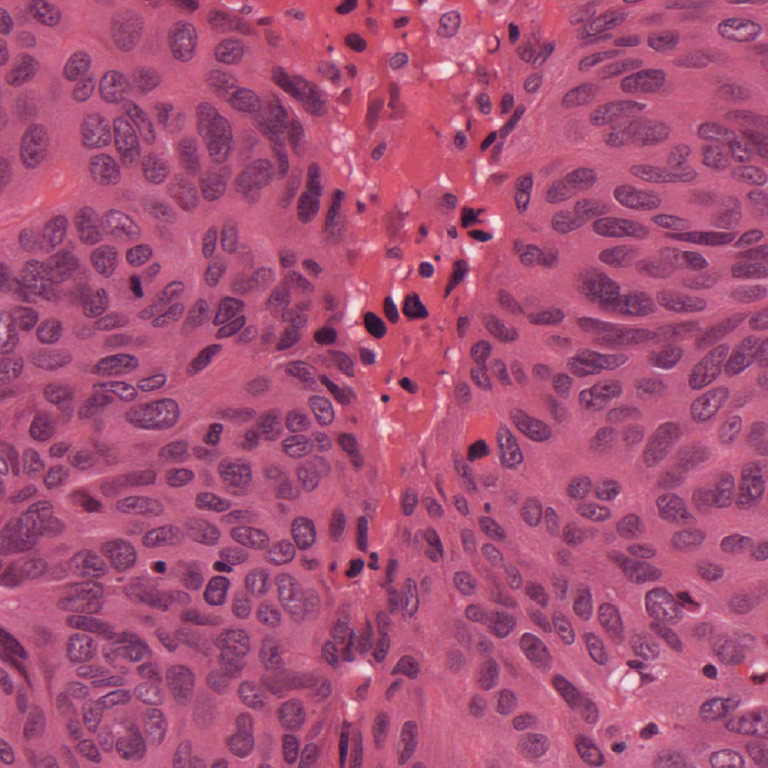
\includegraphics[height=110pt, width=110pt]{segmentaciones/cell1.jpg}}
	\subfigure[$k=80$]{
\includegraphics[height=110pt, width=110pt]{segmentaciones/cell1_seg.jpg}}
	\hspace{3mm}
	\subfigure[]{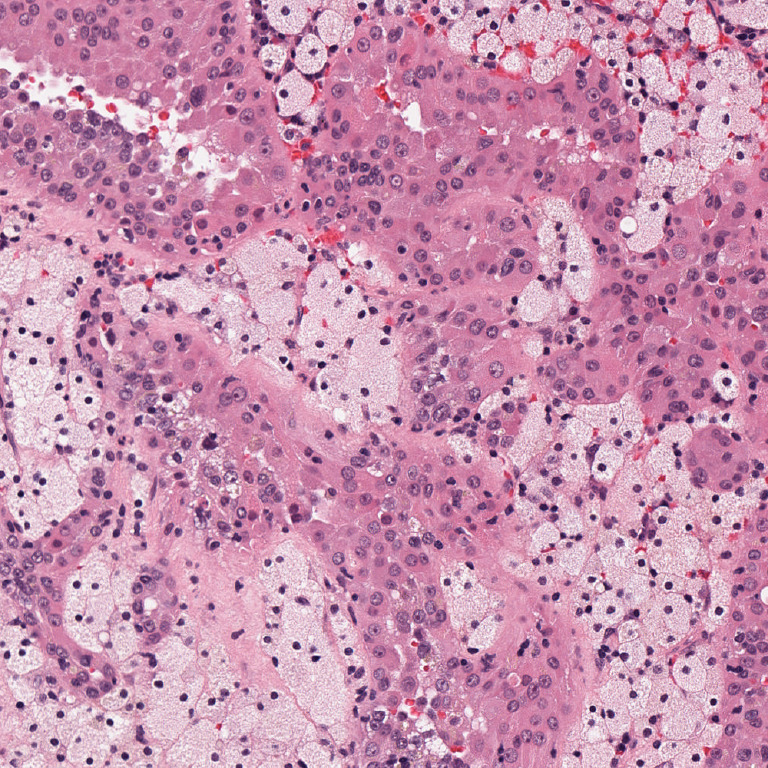
\includegraphics[height=110pt, width=110pt]{segmentaciones/cell2.jpg}}
	\subfigure[$k=1000$]{
\includegraphics[height=110pt, width=110pt]{segmentaciones/cell2_seg.jpg}}
	\caption{}
	\end{center}
\end{figure}
\vspace{-7mm}

\indent Luego de ver las segmentaciones generadas, no hay duda que esta no es una aplicaci\'on viable para el algoritmo. Ambos resultados son incomparables con las im\'agenes originales, haciendo imposible cualquier reconocimiento de secciones relevantes. En definitiva: el algoritmo no es apto para resolver problemas que requieran un alto grado de detalle. 